\newcommand{\addr}[1]{\texttt{#1}}
\newcommand{\pointsto}[0]{\rightarrow}
\newcommand{\union}[0]{\cup}

%Visual debugging can be a valuable method to identify and correct
%errors in simulation software.  Current approaches, however,
%are limited by the traditional workflows ascribed to the \emph{use} of
%simulation software. We endeavor to enable \textit{in situ}
%understanding of simulation data.

%The massive size of current and future data is a cause of great concern
%among the visualization community. \textit{In situ} visualization
%provides one of the most promising approaches for dealing with
%the data deluge.  However, the coupling between visualization and
%simulation tool---including the ongoing maintenance such a coupling
%implies---limits the
%application of \textit{in situ} visualization to a small set of
%technically-inclined users.
%
%This coupling is fundamentally rooted in the exchange of metadata that
%describes the data model and data structures of the simulation code to
%the visualization tool.  In this work, we demonstrate that a data model
%and a simulation program are enough information to fully parameterize
%the data structure metadata for \textit{in situ} visualization,
%obviating the need for coupling code and auxiliary descriptions of data
%arrays and information.

Coupling visualization and analysis software with simulation code is a
resource-intensive task.  As the usage of simulation-based science
grows, we asked ourselves: what would it take to enable \textit{in
situ} visualization for \emph{every} simulation in existence?  This
paper presents an alternative view focusing on the
\textbf{approachability} of
\textit{in situ} visualization.  Utilizing a number of techniques from
the program analysis community and taking advantage of commonalities
in scientific software, we find that we can vastly reduce the time
investment required to achieve visualization-enabled simulations.

\definecolor{darkcyan}{rgb}{0.1,0.5,0.6}
\definecolor{darkgreen}{rgb}{0.1,0.6,0.1}
\lstset{
  commentstyle=\color{darkgreen},
  keywordstyle=\color{red},
  identifierstyle=\color{black},
  keywords="size_t",
  frame=none,
  captionpos=b,
  numbers=none,
  numberstyle=\tiny\color{gray},
}

\section{Introduction}

%\todo{This paper has been accepted, but is still undergoing edits.
%You are reading the author's personal copy.  To obtain the official
%published version, please use the DOI at the bottom left.}

\textit{In situ} visualization has proven to be useful for
simulation-based sciences.  The majority of \textit{in situ}
visualization literature is focused on the performance story: the
growing size of outputs from simulations makes the commonplace
post-processing regime less attractive~\cite{Dorier:2013:Damaris,
Fabian:2011:Catalyst, Whitlock:2011:Libsim}.  While these efforts push
us in the right direction, the impetus is flawed.  The post-processing
approach is not inferior because it scales poorly---though it does
indeed scale poorly---it is
\emph{intrinsically} inferior.  The ability to visualize and understand
a simulation's data as it is generated is \emph{inherently useful}.
The
\textit{in situ} approach has not been ignored until recent years
because it was not useful.  A more likely explanation is that the
difficulty was prohibitive.

Let us redefine `\textit{in situ} visualization' as `interactive
simulation'.  Interactive simulation is simulation that can be
controlled: sped up or slowed down, reinitialized with new parameters,
visualized, selectively refined, or even have its underlying physics
live-edited.  This model of simulation is clearly superior to our
present batch-oriented model.  The cycle time from hypothesis to
verification would be greatly reduced.
%Wasting computational resources
%due to improperly set initial conditions would drop sharply.
%The irony is that the computational resources required to support this
%configuration makes it prohibitively expensive.

% "Get ready, I'm about to unload a whole bunch of 'crazy' on you.  But don't
% worry!" (flip to slide that says "Introduction")  "I'll start off simple."

% I'm glad that compilers can't actually understand source code, because if
% they could mine would say, "wow, you really are batshit crazy, huh?"

% "For example, when I lived in Germany, Google constantly thought I
% spoke fluent German.  Welche ist total falsch, ..."

% If Google (and deep learning in general) has taught us anything, it's that
% it's not important to get things 100% correct---I know, I should have been an
% elementary school math teacher---we just need to get them mostly right and then
% let people fudge the last 3% percent.

% Casts are C's version of a jedi mind trick.

% "You've done ray-casting, you must know ray-tracing, no?" -> "You've ridden a
% bicycle, so you must know how to ride a unicycle, no?"
% "Off-by-one is the difference between success and segfault."
% (on software) "I don't know if I could do stable... but I could do
%   metastable!  That do it for ya?"

% Interactive simulation is good.
%% greatly reduce cycle time
%% much easier to debug
%% amenable to exploratory simulation

% in situ visualization is useful.
%% traditional case
%% understated case: during simulation bringup, debugging.
% coupling visualization and simulation takes much time and effort
% simulation authors may not be experts in data structures, even programming
% simulation-based science is growing in importance, use
% -> we need to make it (much) easier to do in situ visualization

% basic idea: use loop information to tell us about data
% trivial example (listing 1)
% compilation is not lossy!
%% debug information for types
%% dependency information ensures variables are relevant
%% we don't need to recreate the whole program---just these loops!
% model and qualities of the data we search for
% finite state machine for arrays
% detecting accesses (segfaults)
% identifying loops (dominance)
% finding loop induction variable
% visualization itself: GLSL-based 3D volume rendering
% conclusions
% future work
%% distributed memory!
%% support for different data types: 3D arrays are kind of boring
%% "adaptors": 4D data in PsiPhi, in fortran order.
%% connect to more capable vis+a programs (ParaView, VisIt)

Hall et al. note~\cite{Hall:2009:Next50} the importance of ``program-analysis
strategies to improve software construction, maintenance, and
evolution.''  We introduce a methodology for ``0 day'' coupling of
simulation and visualization code.  We remove the need
to link in \emph{any} external code to the simulation.  The simulation
software often does not even need to be recompiled.  The bulk of our
contribution is in the form of program understanding: we demonstrate how to
infer those data that
are interesting \emph{as well as} the parameterization of those data
that enables visualization.  This obviates the need for the simulation
author to conform to or even learn external APIs.

\section{Trivial example}

Consider the task of modifying an existing simulation program to
interactively visualize its in-progress results.  The developer must
identify the primary loop that advances the state of the simulation.
That loop modifies some memory of interest that the developer typically
has some external knowledge about.  The external knowledge generally
revolves around data type and format: `a point cloud of 64-bit floating
point values', for example.  This in turn helps the developer search
for memory matching that organization.  Once the location where the
simulation advances its state is discovered, metadata is uncovered via
a similar process, and a call to the \textit{in situ} visualization
library is inserted.

\begin{lstlisting}[float=*,label=lst:relaxation,language=C,caption=A code
fragment representative of simulation software.  A large array is smoothed
using
a set of nested loops. \texttt{S} is presumed to be a macro that
samples \texttt{data} while properly accounting for edge cases.]
for(size_t j=0; j < dims[1]; ++j) {
  const size_t row = j*dims[0];
  for(size_t i=0; i < dims[0]; ++i) {
    data[row+i] = (S(x-1,y-1) + S(x-0,y-1) + S(x+1,y-1) +
                   S(x-1,y-0) + S(x-0,y-0) + S(x+1,y-0) +
                   S(x-1,y+1) + S(x-0,y+1) + S(x+1,y+1)) / 9.0
  }
}
\end{lstlisting}

The code fragment in Listing~\ref{lst:relaxation} is exemplary of this
task.
The developer adding \textit{in situ} visualization to a 2D
simulation would be pleased to find these loops: the code is accessing
and updating a 2-dimensional structure, `data'.  Next tasks would
be to identify the type and source of the memory in `data'.  Should
it align with the developer's ideas of the simulation's data model,
visualization will be inserted after the loops and testing would be
done.

The work presented here automates this exploratory
search-and-insert-visualization process.

\section{Program model and simulation analysis}
\label{sec:model}

In this section we develop an abstract model of an executing simulation
program.  We will then use this general model to describe a collection
of properties that code such as that in Listing~\ref{lst:relaxation}
follows.  This set of properties codifies the aforementioned developer
process.

%The code fragment in Listing~\ref{lst:relaxation} fits the model of the
%software of interest to us in this work.  Assuming such code is found
%in an environment that greatly emphasizes high-performance implies much
%about the code displayed here.  First, the
%\texttt{data} array can only be a multidimensional array (even though
%its type is one-dimensional).  That array must be heap-allocated using
%a single allocation request: simulations routinely deal with data
%sizes far larger than typical stack or static memory sizes.  Data flow
%analysis would identify
%the access of \texttt{data} within the loops of
%Listing~\ref{lst:relaxation} as dependent on the loop variables
%\texttt{i} and \texttt{j}, though there is little need for such
%formality: both the programmer and the compiler would have strong
%incentives to hoist the access, were this not the case.  Finally,
%\texttt{data}'s dimensionality in this program must be two, and the
%number of elements is $dims[0] \times dims[1]$.

\begin{lstlisting}[label=lst:model,escapechar=!,caption=Definitions for an
abstract machine and analysis based on control flow properties.]
!
\begin{eqnarray}
  BaseType &:=& Booleans \union Integers \union FP
    \union Strings \nonumber\\
  Type &:=& BaseType \union Array \union Pointer \nonumber \\
  Memory &:=& Heap \union Static \union Local
    \union Arguments \union Text \nonumber \\
  IPtr &\in& Text \nonumber\\
  T &:=& Memory \mapsto Type \nonumber \\
  BT &:=& Memory \mapsto BaseType \nonumber \\
  Fqn &:=& [ begin \in Text, end \in Text ]  \mid \ begin < end \nonumber\\
  Where &:=& Text \mapsto Fqn \nonumber \\
  % note that this definition disallows self-modifying code.  that's OK.
  Wr &:=& (m \in Text) \mapsto (n \in (Memory \setminus Text)) \mid m \neq n
    \nonumber\\
	%% turns out we never use the 'Rd' definition.  I guess this would be needed
	%% for denoting data dependencies.  We haven't implemented that yet; unclear
	%% that it's really needed, to be honest.
  %Rd &:=& (m \in Text) \mapsto (n \in (Memory \setminus Text)) \mid m \neq n
  %  \nonumber\\
  %\textbf{class} & \  CFG_{Node} & \  address \  edges \nonumber\\
  \textbf{class} && \  CFG_{Node} \  address \  edges \nonumber\\
  \indent CFG &:=& \{ n \mid n = CFG_{Node} \} \nonumber\\
  BB &:=& Text \mapsto CFG \nonumber \\
  K &:=& Text \mapsto CFG_{Node} \nonumber\\
  Hdr &:=& CFG_{Node} \mapsto Boolean \nonumber\\
  Depth &:=& CFG_{Node} \mapsto Integer \nonumber
 %Q := Text \mapsto F\\
%  \textbf{class} \  ND \  base \  length \  dims \  ndims\\
%  \indent | base \pointsto m \in Heap\\
%  \indent | BT(base) \in FP\\
%  \indent | T(dims) \in Array \union Pointer\\
%  \indent | BT(dims) \in Integer\\
%  \indent | T(ndims) \in Integer\\
%  \indent | ndims > 0\\
%  \indent | Wr(IPtr) \in [ base, base + length ]\\
%  \indent | b \in BB(Where(IPtr)) \land IPtr \notin b \land Hdr(b)
%    \land Depth(K(IPtr)) > Depth(b)\\
\end{eqnarray}
!
\end{lstlisting}

We use the formalisms given in Listing~\ref{lst:model}.  We consider an
abstract machine described by an
\textit{instruction pointer} and the current state of
\textit{memory}.
The instruction pointer advances automatically, and memory
operations consist of reads and writes that map an address to a mutable memory
location.
Note that our definition denies self-modifying code.  Memory is assumed to be
\emph{typed}, with a small set of available types.  The $T$ and $BT$ mappings
define mappings from memory locations to type information.

The running process is assumed to consist of a series of
\textit{functions} ($Fqn$s), that are defined as the functions' upper and
lower addresses.  We make use of an inverse mapping $Where$ that
allows us to identify a function from the
current instruction pointer.
We build local \textit{control flow graph}s (CFGs) that describe the potential
execution paths.  These graphs are represented as a set of \textit{nodes} that
contain an entry \textit{address} as well as a set of \textit{edges}.
We build these CFGs based on the function address range.  We define a
mapping $K$ that allows us to identify a node in the control flow graph
from an instruction address.  We define two final mappings from a node
in the control flow graph: 1)
a predicate identifying \textit{loop headers} ($Hdr$), and 2) a mapping for the
calculated \textit{loop depth} ($Depth$).  In
Listing~\ref{lst:relaxation},
the basic blocks containing \texttt{j < dims[1]} and \texttt{i <
dims[0]} would be the loop headers.  Loop depth is the nesting level of
the provided basic block.  In Listing~\ref{lst:relaxation}, the
assignment to \texttt{row} has a depth of $1$, whereas assignment to
the
element in \texttt{data} has a loop depth of $2$.

Using this model of program execution, we consider the problem of
automatically identifying memory regions that house data that a user
would want to visualize.  We model these as a set of constraints on
type classes.  An instance of the type class allows one to visualize
data within a simulation.

We currently support searching for $N$-dimensional (``ND'') data
arrays.
This type is parameterized by a \texttt{base} address, a
\texttt{length} (in bytes), the number of
dimensions \texttt{ndims}, an array of dimensions \texttt{dims}, and
finally the type of the data.

\begin{eqnarray}
  \indent \textbf{class} \ & ND & \  base \  length \  ndims \  dims \  type
    \nonumber\\
  \indent &\land& \exists m \in Heap : base \pointsto m \\
  \indent &\land& BT(base) = type\\
  \indent &\land& T(dims) \in Array \union Pointer\\
  \indent &\land& BT(dims) \in Integers\\
  \indent &\land& T(ndims) \in Integers\\
  \indent &\land& ndims > 0\\
  \indent &\land& Wr(IPtr) \in [ base, base + length ]\\
  \indent &\land& \exists b \in BB(Where(IPtr)) : \nonumber\\
    && \land \ IPtr \notin b \nonumber \\
    && \land \ Hdr(b) \nonumber\\
    && \land \ Depth(K(IPtr)) > Depth(b)
\end{eqnarray}

We use the $\pointsto$ notation to mean ``points to''; the first
constraint simply states that the data of interest live on the heap.
As simulation data is large, it rarely fits on the stack or even in
statically initialized memory.  The second constraint conveys that the
base type matches a parameter of our model, such as $FP$ (floating
point).  The third and fourth constraints dictate that the dimensions
are stored in a linear list of integers, and the fifth and sixth say
that that the length of that dimension list is a positive integer.

The 7th and 8th constraints are complex and intertwined.  First, the
application must write into the relevant memory block.  Secondly, the
basic block where the data are written must be deeper than another
basic block that contains a loop header.  That is to say that the data
write occurs within a loop.

The formulation gives rise to a pattern matching problem.  The
\texttt{\textbf{class}}es of interest are the patterns, and the space
to match within is the running process' \texttt{Memory}.
In Listing~\ref{lst:relaxation}, the parameter bindings are:
\texttt{data} for \texttt{base}, the size of the allocation (not shown, but
assumed to be \texttt{dims[0]} $\times$ \texttt{dims[1]} $\times$
\texttt{sizeof(float)}) for
\texttt{length}, \texttt{dims} for \texttt{dims}, and $2$ for
\texttt{ndims}.

We do not claim our set of properties is perfect, though they have
proven remarkably effective for our uses thus far.  There are a number
of promising approaches for discovering new invariants
automatically~\cite{Nguyen:2012:Invariants, McCloskey:2010:Infer,
Sharma:2013:DDEC}, as well as low-hanging fruit (e.g. `the memory
is written to a file').  In the future, we wish to allow simulation
authors to specify these constraints at runtime.  The penalty for a lax
specification would be too many visualization windows popping up; the
penalty for too strict a specification would be too few windows popping
up.  The author would see either error almost immediately.

\section{Implementation}

We seek to realize the aforementioned `search' for a given simulation
process.  At first glance static analysis is the best tool for this
task, however it runs into difficulties proving some of the properties.
The pernicious problem is aliasing in C-based languages.  A statement
as
trivial as `\texttt{x = \&y;}' creates two names for the same memory;
thereafter, proving that a write to `\texttt{*x}' changes or does not
change
`\texttt{y}' can be anywhere from unambiguous to undecidable.

A lesser reason to shy away from static analysis is the computational
expense, of which the largest for us is building control flow graphs.
Especially for languages that enjoy methods for exponential code
expansion (e.g. C++ templates), building CFGs for the entire program
would be prohibitively expensive.  A more targeted mechanism is
desirable.

For this and other reasons we utilize static analysis techniques
judiciously sourced by dynamic analysis.  To receive a notification
when a particular memory location is written, we use page protection to
detect writes to it.
Address \addr{0xdeadbeef} is address
\addr{0xdeadbeef}, regardless of the variable name used to access it,
and thus there is no need to solve the aliasing problem.  Control
flow graph construction and analysis are still expensive, but we
isolate their construction to the functions of interest.  By targetting
unstripped binaries that include debug information, we can obtain
robust type information.  Of particular note and perhaps surprise to
many in the scientific visualization community, binary analysis need
not be lossy as compared to source-based
analysis~\cite{Reps:2010:Bottom}.  An advantage of targeting x86-64
machine code is that it is language-agnostic: our framework works for
C++ and Fortran as easily as it works for C, at a fraction of the
implementation costs.

Not all of the $8$ aforementioned properties are worthy of exposition;
variable type information, for example, is straightforwardly sourced
from the binary's debug information.  In the next subsections, we focus
on three of the larger issues: efficiently tracking memory, control
flow graph analysis, and teasing out the dimensions of an array from
the instruction stream of the code accessing it.

\subsection{Memory tracking}

Any heap-allocated memory might potentially be of interest to us.  We
utilize a
\texttt{ptrace(2)}-based supervisor on the target program, and model
each allocation using the finite state machine in
Figure~\ref{fig:fsm}\footnote{\texttt{ptrace} was
consciously chosen for portability.  Previous work relied on
\texttt{LD\_PRELOAD}~\cite{Fogal:2014:Freeprocessing}, and that created
issues porting to some supercomputers.}.  Memory regions begin in
the `null' state and change state based on events observed in the
simulation process.  This event tracking induces overhead, but in the
absence of events simulation execution proceeds at native speeds.

%Our system uses a \texttt{ptrace(2)}-based supervisor for the target
%program.  We induce small changes to process execution that are
%invisible for conformant programs, and our efforts are rewarded through
%efficient notification of events in the simulation.  An example
%event is the access of a data array previously identified as housing
%visualizable data.  While these events induce overhead, in the absence
%of such events, simulation execution runs at native speed.

%Heap-allocated memory is the centerpiece of each
%\texttt{\textbf{class}} we search for.  Any heap-allocated memory
%region is potentially of interest for us, though in real-world programs
%few regions are relevant from a visualization standpoint.  We model
%each memory region by the finite state machine given in
%Figure~\ref{fig:fsm}, with the initial `null' state represented
%implicitly for efficiency reasons.  All memory is assumed to be in the
%`null' state initially.  Memory regions change their state based on
%events observed in the simulation process.  Note that a single event
%may cause a transition in multiple regions.

\begin{figure}
  \centering
  \begin{tikzpicture}[scale=1.0,thick,align=center]
    \node[state](null){null};
    \node[state,right of=null](mloc){malloc};
    \node[state,above of=mloc](mret){mreturn};
    \node[state,right of=mret](allow){allow};
    \node[state,below of=allow](dealloc){dealloc};
    \node[state,below of=dealloc](deny){deny};
    \node[state,left of=deny](hdr){header};
    \path[line](null)--(mloc);
    \path[line](mloc)--(mret);
    \path[line](mret)--(dealloc);
    \path[line](mret)--(allow);
    \path[line](allow)--(dealloc);
    \path[line](allow)--(hdr);
    \path[line](allow) to[out=-20,in=0] (deny);
    \path[line](hdr)--(dealloc);
    \path[line](hdr)--(deny);
    \path[line](hdr) to[out=180,in=120,distance=1cm] (hdr);
    \path[line](deny) to[out=20,in=0] (allow);
    \path[line](deny)--(dealloc);
    \path[line](dealloc) to[out=-200, in=60] (null);
  \end{tikzpicture}

  \caption{Finite state machine governing memory regions of interest.
  Regions transition between the states based on events observed in
  the observed simulation process.  Basic information is obtained in
  the \emph{malloc} and \emph{mreturn} states.  The \emph{allow} state
  initializes parameters for visualization and enables unfettered
  access to the memory. \emph{header} states build up the dimensions of
  the data.  The \emph{deny} state reenables access detection.}
  \label{fig:fsm}

\end{figure}

Allocations cause us to begin tracking a memory region.  We implement
this
event notification using a breakpoint on \texttt{malloc} calls.
By examining the stack and return value, we create a map of the
heap-allocated memory in the process.  Overhead for this operation is
predominantly context switching between the simulation process and our
supervisor.

The \texttt{allow} and \texttt{deny} states solve the access detection
problem.  As mentioned earlier, solving the aliasing problem would
be prohibitively expensive.  Inserting checks at every instruction
that modifies memory is another alternative, but Antoniu and Hatcher
previously demonstrated this
to be too expensive for our needs~\cite{Antoniu:2001:PFault}.  Instead,
we rewrite allocations of interest, enabling write protection on the
returned memory.  This causes the simulation to trap when altering the
data of interest, notifying our supervisor.  To avoid the
performance issue of a notification on \emph{every} access, we catch
only the first per function.

Handling a signal on every dynamic memory access would be prohibitively
expensive.  Therefore we detect the first access within a function
and then allow unfettered memory access until that function returns.
During return, we re-enable protection and execute the defined
visualization steps on the memory.  This assumes the simulation
accesses memory within nested loops instead of accessing the memory via
a functional indirection.  In practice this has not been a problem:
simulations authors are incentivized to access memory in this manner
for performance reasons with or without our supervisor.

%\begin{minipage}{\linewidth}
%\begin{lstlisting}[label=lst:malloc,language=C,caption=Replacement \texttt{malloc} implementation used for tracking field access.]
%void* alignedalloc(size_t n) {
%  void* mem;
%  if(posix_memalign(&mem, getpagesize(), n)
%     != 0) {
%    return NULL;
%  }
%  if(mprotect(mem, n, PROT_READ) != 0) {
%    free(mem);
%    return NULL;
%  }
%  return mem;
%}
%\end{lstlisting}
%\end{minipage}

\subsection{Control flow}

The memory tracking described above enables our supervisor to track
most of the events it needs.  To pinpoint the remaining events we use
analysis based on the local control flow.  When a region is accessed,
we build the local control flow graph for the currently-executing
function.  Our supervisor computes common compiler analysis information
and uses the results to define per-node depth as well as perform loop
header identification,
as shown in Figure~\ref{fig:cfg}.

Our loop header identification relies on the common definitions of
\textit{reachability} and
\textit{dominance}~\cite{Torczon:2007:Compiler}.  Our current algorithm
is
known to be fallible in the presence of harmful \texttt{goto}s, but we
have found it is reliable in practice.  We deem a basic block to be a
loop header when the basic block:
\begin{enumerate}
	\itemsep0em

  \item has exactly 2 in-edges,

	\item has exactly 2 out-edges,

	\item is reachable from one or both out-edges,

	\item is dominated by exactly one in-edge, and

	\item the dominating in-edge does not directly-dominate the other in-edge

\end{enumerate}
In the future, we hope to simplify our flow graphs into loop
trees~\cite{Torczon:2007:Compiler}.  This will resolve some of the
possible ambiguities and modestly improve memory consumption.

We currently use Dyninst's ParseAPI~\cite{Ravipati:2007:Dyninst} to
compute the initial graph, and then perform the analysis with custom
code.  Other tools in this domain are
DynamoRIO~\cite{Bruening:2012:DynamoRIO}, Pin~\cite{Luk:2005:Pin}, and
Valgrind~\cite{Nethercote:2007:Valgrind}.  All of these tools are
capable of sophisticated binary transformations.  However, our needs
are modest and Dyninst presently represents the majority of our
overhead.  In the future we hope to replace this with custom graph
construction code that can more effectively limit computation to the
region of interest.

%Symbol table information aids this process.  The symbol table can provide a
%mapping from \texttt{Text} addresses to functions, for example.

%There are some known limitations to this approach.  One is its
%fragility in the presence of
%\texttt{goto} statements.  If the \texttt{goto} crosses a loop
%boundary, then the depth information calculated may be incorrect, and
%the algorithm will not compute a proper loop tree.  Fortunately, in
%practice this is rare; we have not encountered this case in simulation
%programs of interest.

%Some compiler optimizations pose issues as well.  Loop transformations,
%such as loop tiling or fission, can cause issues with the inference we
%perform.  While it may be possible to workaround these on a case by
%case basis, we reiterate that our use case is primarily in the domain
%of simulation \emph{development}.  As such, these optimizations can
%simply be disabled during development to allow use of the tool.
%
% relies on assumptions:
%%%% data are within the loop because the loop is relevant
%%%% => loop bounds imply bounds on the data
%%%% the application does not use gotos in these tight loops
%%%% loop tiling etc. are not performed
\begin{figure}
  \centering
  \includegraphics[width=\linewidth]{images/dbg/s3}

  \caption{Simplified control flow graph for a small function that
  smooths a 3D array (the 3D analog of Listing~\ref{lst:relaxation}).
  Analysis identifies loop headers and the nesting level (`Depth') of
  each basic block.  On access, the loop tree is traversed to determine
  the dimensionality of the array.}

  \label{fig:cfg}
\end{figure}

\subsection{Symbolic execution}

As described in the $\textbf{class} \ ND$ of Section~\ref{sec:model},
we assume a relation between loop headers and the basic blocks that are
contained within those loops and accessing memory.  The loop variable
must be involved: if it were not, the access would be loop-invariant
and hoisted out of the loop, either explicitly by the programmer or
implicitly by the compiler.  We assume a stronger relation, however:
that the loop conditions imply the dimensionality of the memory regions
accessed therein.

Loop conditionals do not definitively describe the format of the data.
We have however found them to be remarkably accurate, and the loop
nesting to be practically infallible.  Still, we allow the user to
override these discovered bounds, at which point our tool degrades to
only identifying \emph{where} visualization should be performed.  More
work is needed in this area.

Our general approach is to differentiate the loop bound from the
induction variable in the loop conditional.
Listing~\ref{lst:header} gives the basic block for a real-world loop
conditional (what might be implemented for \texttt{i < dims[0]}):

\begin{lstlisting}[label=lst:header,caption=Instructions within a
sample loop header.  The induction variable and the loop bound
appear as arguments to the \texttt{CMP} instruction.]
  MOV %rdx, [%rip+0x20507]
  MOV %rax, [%rpb-0x60]
  CMP %rdx, %rax
  JB -0x275
\end{lstlisting}

We would like to know which of \texttt{\%rdx} and \texttt{\%rax} in
Listing~\ref{lst:header} is the loop bound.  Unfortunately a myopic
view of
the \texttt{CMP} instruction is insufficient for operand
classification: the \emph{source} of the values is
in the two \texttt{MOV} instructions.
We use Algorithm~\ref{alg:sinterp} to track the source of operands by
interpreting each instruction in the basic block.  A heuristic that the
induction variable is a local variable is used to differentiate the
loop bound from the induction variable.

\begin{algorithm}

  \caption{Tracking virtual register sets to identify the source
  of data.  The algorithm begins at a loop header basic block and
  symbolically executes each instruction.  The resultant data structure
  can be used to query the source of an instruction operand's value.}

%  These sources are then
%  used to lookup debug information and interpret register contents.
  \label{alg:sinterp}
  \begin{algorithmic}[1]
    \State register[*] := UNKNOWN
    \State instruction := bb$_{addr}$ \Comment first instruction in loop header
    \Repeat \Comment foreach instruction in the basic block
      %\State \Comment cast to instruction of appropriate type
      \If{instruction.Opcode = MOV}
        \State mov := (MovInstruction)instruction
        \If{mov.source $\in$ register}
          \State register[mov.target] := register[mov.source]
        \ElsIf{mov.source $\in Memory$}
          \State register[mov.target] := mov.source +\\
                            \hspace{14.4em} memdiff[mov.source]
        \EndIf
      \EndIf
      \If{instruction.Opcode = ADD} \Comment track $\Delta$addr
        \State add := (AddInstruction)instruction
        \If{add.dest $\in$ register $\land$
            register[add.dest] $\neq$ UNKNOWN}
          \State register[add.dest] += add.source
        \EndIf
        \If{add.dest $\in Memory$}
          \State memdiff[add.dest] += add.source
        \EndIf
      \EndIf
			\State \Comment ... SUB, MUL, etc. cases omitted for brevity
      \State instruction := next(instruction)
    \Until instruction.Opcode = CMP
  \end{algorithmic}
\end{algorithm}

It is not strictly true that induction variables must be local
variables.  However, we have only seen this assumption violated in
artifically-constructed test programs.  Data dependency information and
def/use sets~\cite{Torczon:2007:Compiler} should make this more robust
in the future.

Each iteration of this process gives a single loop bound.  By following
the
state machine in Figure~\ref{fig:fsm} and setting breakpoints up the
chain of the loop tree, we derive the full set of bounds.  At the
function boundary, we enter the `deny' state and re-enable memory
protection for that region.

% Integer-based or pointer-based indices/bounds present a problem for us
% currently.  In future, use type to discern?

\subsection{Visualization}

Our contribution is in the approach to program understanding, though
rendering is required to demonstrate these aspects. We have implemented
a simple GLSL-based volume renderer and a
python-based \texttt{yt}~\cite{Turk:2010:yt} backend thus far.
Figure~\ref{fig:volren} shows the former with data sourced from a
combustion simulation.  In the future, we hope to incorporate backends
using established visualization tools such as ImageVis3D, VisIt, and/or
ParaView~\cite{Fogal:2010:Tuvok, Childs:2012:VisIt,
Ahrens:2005:ParaView}.

\begin{figure}
  \includegraphics[width=\linewidth]{images/dbg/psiphi}

%  \caption{Volume rendering of the volume of tissue activated from
%  a biomedical simulation of deep brain stimulation.  Array shape
%  information and data were read from the running simulation and
%  serialized to disk, while a concurrent process made the data suitable
%  for import into a volume rendering tool.  No user intervention was
%  required, beyond setting the transfer function to derive the color
%  information.}

  \caption{Volume rendering of the temperature field from a
  \textit{PsiPhi} simulation~\cite{Proch:2014:PsiPhi}.  Array shape
  information and data were pulled from the running simulation and
  given to an \textit{ad hoc} volume renderer.  Instrumentation and
  rendering time is on the order of milliseconds whereas a timestep
  can take seconds.  User interaction was limited to transfer function
  design.}

  \label{fig:volren}
\end{figure}

\subsection{Performance}
\label{sec:performance}

Performance is a cause for concern, as our instrumentation's
theoretical upper
bound is on par with \texttt{valgrind}-level
instrumentation~\cite{Nethercote:2007:Valgrind}.  Fortunately, in
practice we have found the slowdown to be approximately 4x for
real-world programs.  There is much work still to be done in this
regard: the largest
limitation is that we currently visualize \emph{every} timestep's
results.

Figure~\ref{fig:performance} looks at multiple aspects of performance
across this set of programs.  The red `Uninstrumented' bar represents
an upper bound on performance.  `Trace' inserts breakpoints at
`\texttt{malloc}', `\texttt{free}', and their return addresses,
measuring what it costs to start and stop the execution of the
simulation program.  Simulations that utilize more regions of dynamic
memory will see higher overheads due to this aspect.  However, the
graph does not capture the phased nature of these processes: generally,
our instrumentation is heavy for allocation-heavy startup routines and
lightweight thereafter.

%  As simulation sizes increase, the initialization phase holds
%constant whilst the compute phase scales polynomially.

\begin{figure}
  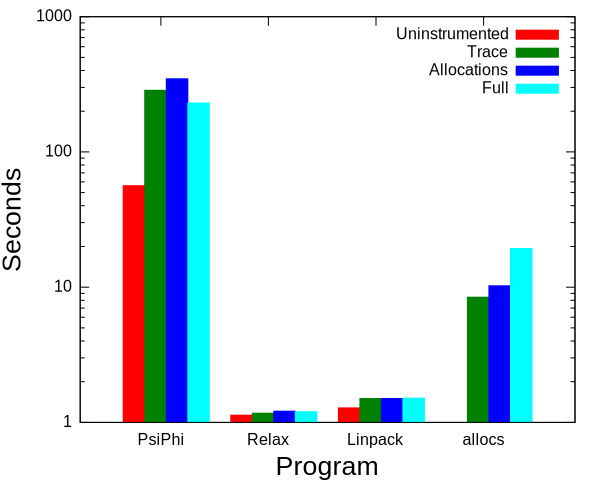
\includegraphics[width=\linewidth]{images/dbg/mtrace/performance}

  \caption{Performance of our evaluation programs under different
  instrumentation scenarios. Note logarithmic scale.  `Uninstrumented'
  is the runtime of the simulation without our interference. `Trace'
  interrupts for allocations; `Allocations' \emph{reports} allocations
  as well, which requires reading more data from the instrumented
  program.  `Full' does allocation tracking, access detection,
  analysis, and visualization of the data.}

  \label{fig:performance}
\end{figure}

Figure~\ref{fig:performance}'s `Relax' and `allocs' are artificial
programs constructed to illustrate overheads.  The
main component of `Relax' is Listing~\ref{lst:relaxation}. `allocs'
does nothing but allocate memory, the worst case for our
instrumentation.  We note that real-world programs experience
considerably lower overheads, with the popular Linpack seeing a modest
15\% slowdown.

\textit{Linpack} is the matrix-vector multiplication benchmark of
floating point performance that is used to rank supercomputers in the
popular `Top500' list. \textit{Relax} is a program that identifies
the steady state for the case of a plane connected to a constant heat
source.  The program's ratio between function calls and accessing the
data to be visualized is at parity, stressing the memory access and
analysis aspects of our supervisor. \textit{PsiPhi} is a real-world
computational fluid dynamics solver that focuses on Large Eddy
Simulation (LES) of flows that include combustion and other types of
chemical reactions~\cite{Proch:2014:PsiPhi}. \textit{allocs} is a test
program that simply allocs and frees memory without ever acessing it.

`Allocations' is a more expensive variant of the `Trace' benchmark.
In addition to allocation interception, this version reads relevant
information from the client process so that it may generate a report
of the [de]allocations made by the process.  The traces this algorithm
creates might be useful in producing and analyzing heap usage over
time, in the same manner as Valgrind's
`Massif'~\cite{Nethercote:2006:Massif}.  We note that this adds little
additional overhead to the instrumentation, demonstrating that reading
memory from the process is cheap.

%`Full' in
%Figure~\ref{fig:performance} details overheads for the full gamut of
%our analysis techniques.  Conflating the results, however, are filters
%that can be applied when more analysis is performed.  As one example of
%these
%filters, `Full' identifies the caller of \texttt{malloc} and ignores
%the allocation if the
%memory is an internal \textit{glibc} buffer.  With the extra
%information gained from this additional work, `Full' can in many
%cases realize that an allocation region is not interesting.  It then
%removes the item from the set of memory it tracks, thereby reducing the
%overhead induced.  If the overhead of tracking the memory exceeds that
%of the analysis, then this variant will actually be cheaper than the
%more na\"ive implementations.

In practical terms, the performance scales with 1) the number of
allocations the program performs, and 2) the number of allocations that
are tracked and provide source locations for analysis.  Reducing the
number of allocations requires changing the programs of interest, which
is counter to our goal of a transparent solution.  However, avoiding
the tracking infrastructure for memory that the user is not interested
in is a plausible practical mechanism by which the user can influence
the performance of the instrumented system.

%\section{Related work}
%
%Debugging high-performance computing applications is especially important as
%parallelism increases and debugging becomes correspondingly more difficult.
%\cite{Laguna:2011:Debugging} extend their earlier
%work~\cite{Bronevetsky:2010:AutomaDeD} with a scalable method to
%identify divergent parallel processes based on reduced control flow and
%call stack information. Gao et al.~\cite{Gao:2007:DMTracker} watch
%data movement patterns of a parallel application and use anomalies to
%statistically infer a set of undesirable program activites.
%\cite{Luecke:2003:MPICheck} instruments an MPI program to detect
%invalid or inconsistent usage of the library.  All of these debugging
%techniques are focused on identifying and eliminating the source of
%programming-level errors, such as data corruption, deadlock, or
%livelock.  In contrast, our \textit{ad hoc} visualization approach
%would be more appropriate to identify algorithmic errors, such as
%non-convergent error smoothing.
%
%\cite{Rosenblum:2011:Authors} use program control flow graphs and a
%custom-defined set of stylistic considerations to classify programs by
%their authors given only the input binary.
%\cite{Bernat:2012:BinEdit} define a number of `safe' control flow graph
%transformations and an algebra for describing and deriving new ones.
%Our code injection for page-aligned allocation is straightforward and
%undeserving of such a robust formalism.
%
%Our approach must identify and verify memory regions and related
%variables that meet a set of invariants. McCloskey et
%al.~\cite{McCloskey:2010:Infer} provided both a language and an
%implementation to specify complex invariants suitable for our analyses.
%\cite{Nguyen:2012:Invariants} use dynamic analysis to identify detailed
%invariants that include array accesses.  Our approach utilizes
%invariants that include reasoning at different levels, such as control
%flow, in addition to invariants like those discovered therein.
%\cite{Sharma:2013:DDEC} implement equivalence identification for
%instruction-level loops.  Our code injection and access detection might
%be seen as a lighter weight variant of their sandboxing technique.  The
%techniques in~\cite{Sharma:2013:DDEC} present a potential vector
%for inferring bounds from pointer-based loop guards, by deriving
%equivalent index-based guards and relying on our existing analysis
%infrastructure.

\section{Conclusions}

We have elucidated a method and demonstrated a prototype that
eliminates the surface area between simulation code and visualization
tool.  By recovering the loop structure of a target binary and
carefully instrumenting memory accesses, one can automatically insert
visualization at appropriate places in a running simulation.

%The major drawbacks at present are related to data types and data
%decomposition.  Presently we support only a single kind of simulation
%data: $N$-dimensional arrays.  While these have proven popular,
%they are far from universal.  Extending to other data types may be
%nontrivial.  A larger problem is data decomposition: we do not consider
%distributed-memory parallel simulations at present, and it seems likely
%that automatically reconstructing the full domain from its distributed
%pieces is undecidable.  User annotations may help in this endeavor.

\subsection{Future work}

The most glaring present omission is the lack of support for data
types beyond regular $N$-dimensional grids.  An obvious next target
is related data types such as adaptive mesh refinement data.
Curvilinear grids may prove simple as well, and meshes or point clouds
would certainly be of interest.  An area of uncertainty is in data
decomposition in distributed memory simulations.

We do not seek to replicate the full functionality of tools like
VisIt or ParaView.  We must therefore couple with one of these tools;
doing so would immediately increase the utility of our prototype
implementation.

We make a number of assumptions that are practically but not strictly
true.  Each requires more investigation, and aspects such as the
specification used in our search require more user control than we
presently have made available.

While some of these issues involve significant engineering efforts,
the work presented here demonstrates that there is no need to modify
simulation code to
inject \textit{in situ} visualization.  We hope this encourages others
to pursue 0-modification approaches to \textit{in situ} visualization.

%The astute reader may note that memory protection is possible only on
%page-aligned data.  We therefore require a modified \texttt{malloc}
%implementation that calls \texttt{posix\_memalign} (to allocate the
%page-aligned memory) followed by \texttt{mprotect} (to set up the
%desired memory protections).  Since we do not require the user to link
%against any runtime, adding a function in the traditional way is not
%viable.  Instead, we inject our modified \texttt{malloc} implementation
%directly into the executing process image after static initialization
%has completed.  We modify the instruction pointer when a
%\texttt{malloc} occurs to instead jump to our page protection
%allocation routine.

%\section{Related work}
%
%\textit{In situ} visualization has a rich history in the visualization
%community.  Recent frameworks include Damaris/Viz, the ParaView
%Coprocessing library, and VisIt's `libsim'~\cite{Dorier:2013:Damaris,
%Fabian:2011:Catalyst, Whitlock:2011:Libsim}. Dorier et
%al.~\cite{Dorier:2013:Damaris} open
%by noting the important factors for an \textit{in situ} visualization
%tool. Among these factors are \textbf{low impact on code} and
%\textbf{low impact on runtime}.  As our solution requires zero code
%modifications, it has the lowest impact on the simulation code of any
%\textit{in situ} visualization tool.  Performance is viable in
%favorable conditions, and we hope to lower the overhead in the future.
%
%Debugging high-performance computing applications is especially important as
%parallelism increases and debugging becomes correspondingly more difficult.
%\cite{Laguna:2011:Debugging} extend their earlier
%work~\cite{Bronevetsky:2010:AutomaDeD} with a scalable method to
%identify divergent parallel processes based on reduced control flow and
%call stack information. Gao et al.~\cite{Gao:2007:DMTracker} watch
%data movement patterns of a parallel application and use anomalies to
%statistically infer a set of undesirable program activites.
%\cite{Luecke:2003:MPICheck} instruments an MPI program to detect
%invalid or inconsistent usage of the library.  All of these debugging
%techniques are focused on identifying and eliminating the source of
%programming-level errors, such as data corruption, deadlock, or
%livelock.  In contrast, our \textit{ad hoc} visualization approach
%would be more appropriate to identify algorithmic errors, such as
%non-convergent error smoothing.
%
%\cite{Rosenblum:2011:Authors} use program control flow graphs and a
%custom-defined set of stylistic considerations to classify programs by
%their authors given only the input binary.
%\cite{Bernat:2012:BinEdit} define a number of `safe' control flow graph
%transformations and an algebra for describing and deriving new ones.
%Our code injection for page-aligned allocation is straightforward and
%undeserving of such a robust formalism.
%
%Our approach must identify and verify memory regions and related
%variables that meet a set of invariants. McCloskey et
%al.~\cite{McCloskey:2010:Infer} provided both a language and an
%implementation to specify complex invariants suitable for our analyses.
%\cite{Nguyen:2012:Invariants} use dynamic analysis to identify detailed
%invariants that include array accesses.  Our approach utilizes
%invariants that include reasoning at different levels, such as control
%flow, in addition to invariants like those discovered therein.
%\cite{Sharma:2013:DDEC} implement equivalence identification for
%instruction-level loops.  Our code injection and access detection might
%be seen as a lighter weight variant of their sandboxing technique.  The
%techniques in~\cite{Sharma:2013:DDEC} present a potential vector
%for inferring bounds from pointer-based loop guards, by deriving
%equivalent index-based guards and relying on our existing analysis
%infrastructure.
